% vim:ft=tex:
%
\documentclass[class=article,border=1pt]{standalone}
\usepackage{amsmath}

\usepackage{tikz}
\usetikzlibrary{calc,angles,positioning,intersections}
\usepackage[cm]{sfmath}
% \usepackage[T1]{fontenc}
\renewcommand{\familydefault}{\sfdefault}
% \fontfamily{Linux Biolinum O}\selectfont


\usepackage{pgfplots}
\pgfplotsset{compat=1.11}

\begin{document}
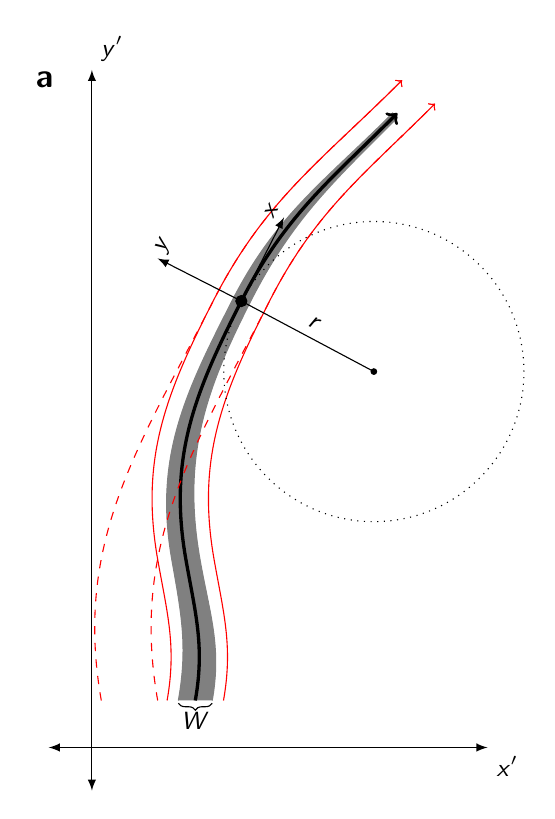
\begin{tikzpicture}
\begin{axis}[width=4.9in,axis equal image,clip=false,
axis lines=middle,
xmin=-0.25,xmax=4,
xlabel=$x'$,ylabel=$y'$,
ymin=-0.25,ymax=7,
restrict y to domain=-54:90,
enlargelimits={abs=0.25cm},
axis line style={latex-latex},
ticklabel style={font=\tiny,fill=white},
xtick={\empty},ytick={\empty},
extra x ticks={15},
extra x tick labels={15},
xticklabel style={anchor=south},
xticklabel shift=-4pt,
extra y ticks={15},
extra y tick labels={15},
yticklabel style={anchor=west},
yticklabel shift=-4pt,
xlabel style={at={(ticklabel* cs:1)},anchor=north west},
ylabel style={at={(ticklabel* cs:1)},anchor=south west}
]

\node(a) at (-0.5, 7.1){\large\bf a};
\small
% Flowline
\filldraw[gray] (0.92,0.5) to [out=80, in=280] (0.85,2.0) to [out=100, in=243] (1.49,4.75) to [out=63, in=225] (3.2,6.75) -- (3.25,6.7) to [out=225, in=63] (1.69,4.75) to [out=243, in=100] (1.15, 2.0) to [out=280, in=80] (1.28,0.5);
\draw[->, very thick, black] (1.1,0.5) to [out=80, in=280] (1.0, 2.0) to [out=100, in=243] (1.59,4.75) to [out=63, in=225] (3.25,6.75);
\draw[decoration={brace,mirror,raise=1pt},decorate] (0.92,0.5) -- node[below=1pt] {$W$} (1.28,0.5);


% ice stream
\draw[->, thin, red] (1.4,0.5) to [out=80, in=280] (1.3, 2.0) to [out=100, in=243] (1.89,4.75) to [out=63, in=225] (3.65,6.85);
\draw[->, thin, red] (0.8,0.5) to [out=80, in=280] (0.7, 2.0) to [out=100, in=243] (1.29,4.75) to [out=63, in=225] (3.3,7.1);
\draw[->, thin, red, dashed] (0.7,0.5) to [out=100, in=243] (1.89,4.75) to [out=63, in=225] (3.65,6.85);
\draw[->, thin, red, dashed] (0.1,0.5) to [out=100, in=243] (1.29,4.75) to [out=63, in=225] (3.3,7.1);

% circle for r
\filldraw [black] (1.59,4.75) circle (2pt);
\draw[thin, black, dotted] (4.597,4) arc (0:360:1.597);
\draw[thin, black] (3.0, 4) -- (1.59, 4.75)node[pos=0.5,above,sloped]{$r$};
\filldraw [black] (3,4) circle (1pt);

% x-y axis
\begin{scope}[rotate around={63:(1.59,4.75)},draw=black]
    \draw[-latex] (1.59,4.75) -- (2.59,4.75);
    \draw[-latex] (1.59,4.75) -- (1.59,5.75);
    \node(x) at (2.59,4.9)[rotate=63]{$x$};
    \node(y) at (1.74,5.75)[rotate=63]{$y$};
\end{scope}
\end{axis}
\end{tikzpicture}

\begin{tikzpicture}
\begin{axis}[width=4.9in,axis equal image,clip=false,
axis lines=middle,
xmin=-2.25,xmax=2.25,
xlabel=$x$,ylabel=$z$,
ymin=-0.5,ymax=3,
restrict y to domain=-54:90,
enlargelimits={abs=0.25cm},
axis line style={latex-latex},
ticklabel style={font=\tiny,fill=white},
xtick={\empty},ytick={\empty},
extra x ticks={15},
extra x tick labels={15},
xticklabel style={anchor=south},
xticklabel shift=-4pt,
extra y ticks={15},
extra y tick labels={15},
yticklabel style={anchor=west},
yticklabel shift=-4pt,
xlabel style={at={(ticklabel* cs:1)},anchor=north west},
ylabel style={at={(ticklabel* cs:1)},anchor=south west}
]
\node(b) at (-2, 3){\large\bf b};
\small
\draw[latex-latex] (0.25,0.75) -- (-0.25,-0.75)node[pos=0.0,right]{$y$};

% Surface
\draw[very thick, black] (-2.0,2.5) to [out=0, in=180] (2.0, 1.5);
% Bed
\draw[very thick, black] (-2.0, 0.75) to [out=360, in=180] (0.0, -0.1) to [out=0,in=180] (2.0, 0.25);
\node(bed) at (-1.5, 0.25){Bed}; 
% \node(ice) at (1.0, 1.5){Ice}; 

\draw[thin, black] (1.75, 0.27) -- (1.75, 1.48)node[pos=0.5, right]{$H$};
\draw[thin, black] (1.7, 0.27) -- (1.8, 0.27);
\draw[thin, black] (1.7, 1.48) -- (1.8, 1.48);


\draw[->] (-1.5, 2.5) -- (-1.0, 2.5)node[above]{$u_s$};

\draw[->] (-1.5, 1.5) -- (-1.0, 1.5)node[above]{$u$};
\draw[->] (-1.5, 1.5) -- (-1.5, 2.0)node[left]{$w$};
\draw[->] (-1.5, 1.5) -- (-1.375, 1.875)node[right]{$v$};

\end{axis}
\end{tikzpicture}
\end{document}
